% 03_perturbations.tex
\section{Linear perturbations and the Boltzmann hierarchy}
\label{ch:perturbations}

The CMB anisotropy is a measurement of small perturbations to the homogeneous background of chapter 1. To compute it we need to linearise the Einstein equations around the FRW background and evolve a coupled system: metric perturbations $+$ density and velocity perturbations of every species (CDM, baryons, photons, neutrinos). For photons (and neutrinos before they decouple) the situation is richer than for a pressure-free fluid: we need to evolve the distribution function, which depends on direction as well as position. The standard treatment expands the directional dependence in Legendre polynomials, producing a coupled ladder of multipoles -- the Boltzmann hierarchy.

This is the longest chapter in the tutorial. Every equation has a physical meaning, and the structure of the code follows the structure of the equations one-for-one.

\subsection{Linearised FRW: scalar perturbations}

Write the metric as
\[
  g_{\mu\nu} = \bar g_{\mu\nu} + a^2(\tau)\, h_{\mu\nu},
\]
with $\bar g_{\mu\nu}$ the FRW background of chapter 1 (now in conformal time, with $\bar g_{\mu\nu} = a^2(\tau)\,\mathrm{diag}(-1,1,1,1)$) and $h_{\mu\nu}$ a small perturbation. By the SVT decomposition, $h_{\mu\nu}$ splits into two scalar, two vector, and two tensor degrees of freedom under spatial rotations. Scalar perturbations are what we need now; tensors appear in chapter 7; vectors decay and we ignore them.

Two gauges are in common use.

\paragraph{Synchronous gauge} (used in CAMB and in our code). Set $h_{00} = h_{0i} = 0$, leaving only spatial perturbations:
\begin{equation}
  \mathrm{d}s^2 = a^2(\tau)\bigl[-\mathrm{d}\tau^2 + (\delta_{ij} + h_{ij})\,\mathrm{d}x^i \mathrm{d}x^j\bigr].
  \label{eq:synch_gauge}
\end{equation}
For scalar perturbations $h_{ij}$ is built from two functions $h$ (trace) and $\eta$ (longitudinal), parametrised in Fourier space by
\[
  h_{ij}(\vec k, \tau) = \hat k_i \hat k_j\, h(\vec k, \tau) + (\hat k_i \hat k_j - \tfrac{1}{3}\delta_{ij})\, 6\eta(\vec k, \tau).
\]
Synchronous comoving observers (those at rest at $\tau = 0$ in this coordinate system) follow geodesics. There is a residual gauge freedom; we fix it by setting cold dark matter to be at rest in this gauge.

\paragraph{Conformal Newtonian gauge.}
\[
  \mathrm{d}s^2 = a^2(\tau)\bigl[-(1 + 2\Psi)\,\mathrm{d}\tau^2 + (1 - 2\Phi)\,\delta_{ij}\,\mathrm{d}x^i \mathrm{d}x^j\bigr],
\]
with $\Phi$ the curvature perturbation and $\Psi$ the gravitational potential. These two are gauge-invariant. The combination
\[
  \Psi_W \equiv \tfrac{1}{2}(\Phi + \Psi)
\]
is the \emph{Weyl potential}; this is what deflects photons in gravitational lensing (chapter 6).

For the rest of this chapter we work in synchronous gauge. We will not need the Newtonian-gauge form, except that the Weyl potential will be reconstructed from synchronous-gauge variables in chapter 6.

\subsection{Einstein equations for $h$ and $\eta$}

Linearising the Einstein equations around the FRW background in synchronous gauge produces four scalar equations (00, $0i$, trace, traceless). Only two combinations are independent; the other two are conservation laws. The conventional choice (Ma \& Bertschinger 1995) is
\begin{align}
  k^2 \eta - \tfrac{1}{2}\mathcal{H}\,\dot h &= 4\pi G a^2\, \delta\rho, \label{eq:Einstein00}\\
  k^2 \dot\eta &= 4\pi G a^2 (\rho + p)\,\theta, \label{eq:Einstein0i}\\
  \ddot h + 2 \mathcal{H} \dot h - 2 k^2 \eta &= -8\pi G a^2\, \delta p\,(\text{trace}), \\
  \ddot h + 6 \ddot\eta + 2\mathcal{H}(\dot h + 6 \dot\eta) - 2 k^2 \eta &= -24\pi G a^2 (\rho + p)\sigma_\text{anis},
\end{align}
where $\delta\rho = \sum_i \delta\rho_i$, $(\rho + p)\theta = \sum_i (\rho_i + p_i)\theta_i$, etc. are sums over species, and $\sigma_\text{anis}$ is the anisotropic stress (non-zero for photons and neutrinos with non-trivial quadrupole). The conformal-time Hubble parameter is $\mathcal{H} = \dot a/a = aH$.

A useful intermediate variable is the metric shear
\[
  \sigma = \frac{\dot h + 6 \dot\eta}{2k},
\]
which appears constantly in the equations of motion below.

\subsection{The fluid sector: CDM and baryons}

For pressure-free CDM (cold dark matter), the linearised continuity and Euler equations in synchronous gauge are
\begin{align}
  \dot\delta_c &= -\tfrac{1}{2}\dot h, \label{eq:cont_c}\\
  \dot\theta_c &= 0\quad (\text{gauge choice: CDM at rest}). \label{eq:euler_c}
\end{align}
For baryons,
\begin{align}
  \dot\delta_b &= -\theta_b - \tfrac{1}{2}\dot h, \label{eq:cont_b}\\
  \dot\theta_b &= -\mathcal{H}\theta_b + c_s^2 k^2 \delta_b + \frac{\dot\kappa}{R}(\theta_\gamma - \theta_b), \label{eq:euler_b}
\end{align}
where $R = (3/4)\rho_b/\rho_\gamma$ is the baryon-photon momentum ratio, $c_s^2$ is the baryon sound speed, and the last term is Thomson drag from the photons.

These come straight from $\nabla_\mu T^{\mu\nu} = 0$ for each species, linearised around FRW. The metric perturbation $h$ enters as a source because the metric expansion contributes to density dilution.

\subsection{The photon distribution function}

The photon phase-space density $f_\gamma(\vec x, \vec p, \tau)$ depends on direction, so we cannot just track density and velocity. Two simplifications help:
\begin{itemize}
  \item For massless particles, $p_0 = |\vec p|$, and the temperature shift $\delta T/T$ does not depend on $|\vec p|$ (the Boltzmann equation conserves blackbody form, just at varying $T$). So we can integrate $f_\gamma$ over $|\vec p|$ and work with a function of direction only.
  \item For scalar perturbations, the only preferred direction is the wavevector $\hat k$. So the temperature perturbation depends on the photon direction $\hat n$ only through $\mu = \hat k \cdot \hat n$.
\end{itemize}
We thus expand
\[
  \frac{\delta T_\gamma}{T}(\vec k, \hat n, \tau) = \sum_\ell (-i)^\ell (2\ell + 1)\, \Theta_\ell(\vec k, \tau)\, P_\ell(\mu).
\]
The relativistic notation often uses different variables: $\delta_\gamma = 4\Theta_0$, $q_\gamma = (4/3)\theta_\gamma/k = 4\Theta_1$, $\pi_\gamma \propto \Theta_2$, etc. Our code follows the CAMB convention and stores $\delta_\gamma$, $q_\gamma$, $\pi_\gamma$, and the higher $\Theta_\ell$.

\begin{aside}[Why Legendre polynomials]
The Boltzmann streaming term $\mu \cdot \partial_x f$ in Fourier space becomes multiplication by $\mu$. The recursion
\[
  \mu P_\ell(\mu) = \frac{\ell}{2\ell + 1} P_{\ell-1}(\mu) + \frac{\ell + 1}{2\ell + 1} P_{\ell + 1}(\mu)
\]
turns this into a tridiagonal coupling among adjacent multipoles $\Theta_{\ell-1}, \Theta_\ell, \Theta_{\ell+1}$. This is the origin of the ``hierarchy'' -- a ladder of equations that streams power from low to high multipoles.
\end{aside}

\subsection{The Boltzmann hierarchy for photons}

Plugging the Legendre expansion into the Boltzmann equation and applying the recursion, plus including Thomson scattering off electrons, gives the photon hierarchy in synchronous gauge:
\begin{align}
  \dot\delta_\gamma &= -\tfrac{4}{3}k\theta_\gamma\cdot\tfrac{3}{4k} \cdot k - \tfrac{2}{3}\dot h, \nonumber\\
                    &= -k\, q_\gamma - \tfrac{2}{3}\dot h, \label{eq:dot_delta_gamma}\\
  \dot q_\gamma &= \tfrac{k}{3}\,(\delta_\gamma - 2 \pi_\gamma) - \dot\kappa\,(q_\gamma - \tfrac{4}{3}\theta_b/k), \label{eq:dot_q_gamma}\\
  \dot\pi_\gamma &= \tfrac{2}{5}k\, q_\gamma - \tfrac{3}{5}k \Theta_3 - \dot\kappa(\pi_\gamma - \Pi) + \tfrac{8}{15}k\sigma, \label{eq:dot_pi_gamma}\\
  \dot\Theta_\ell &= \frac{k}{2\ell+1}\Bigl[\ell\,\Theta_{\ell-1} - (\ell+1)\,\Theta_{\ell+1}\Bigr] - \dot\kappa\,\Theta_\ell, \quad \ell \geq 3. \label{eq:Theta_hierarchy}
\end{align}
The polarisation source $\Pi = (\pi_\gamma + 9 E_2/5)/10$ couples the temperature quadrupole to the $E$-mode polarisation quadrupole through Thomson scattering. The metric shear $\sigma$ enters the quadrupole equation through the linearised tetrad rotation; this is what couples the $\ell = 2$ moment back to the background gravity.

The hierarchy is truncated at $\ell_\mathrm{max} \approx 15$ for photons with a free-streaming closure
\[
  \dot\Theta_{\ell_\mathrm{max}} = k\,\Theta_{\ell_\mathrm{max} - 1} - (\ell_\mathrm{max} + 1)\,\tau^{-1}\, \Theta_{\ell_\mathrm{max}} - \dot\kappa\,\Theta_{\ell_\mathrm{max}}.
\]

\subsection{$E$-mode polarisation}

Polarisation is generated by Thomson scattering of an anisotropic radiation field. The Boltzmann equation for the $E$-mode multipoles follows the same Legendre-recursion structure but with a different geometric prefactor reflecting the spin-2 nature of polarisation:
\begin{align}
  \dot E_2 &= -\dot\kappa(E_2 - \Pi) - \tfrac{k}{3}E_3, \\
  \dot E_\ell &= -\dot\kappa\, E_\ell + \frac{k\,\ell}{2\ell+1}E_{\ell-1} - \frac{k\,(\ell + 3)(\ell - 1)}{(\ell + 1)(2\ell + 1)} E_{\ell + 1}, \quad \ell \geq 3.
\end{align}
The Thomson source $-\dot\kappa(E_2 - \Pi)$ generates $E$-mode amplitude from the quadrupole; the streaming term pumps power up the hierarchy. There are no $B$-modes from scalar perturbations -- a parity argument: scalar perturbations only have $\hat k$ to break direction, and $\hat k$ is parity-even.

\subsection{Massless neutrinos}

The same Boltzmann hierarchy applies, with $\dot\kappa = 0$ (no scattering after $T \approx 1\,\mathrm{MeV}$):
\begin{align}
  \dot\delta_\nu &= -\tfrac{4}{3}k\, q_\nu - \tfrac{2}{3}\dot h, \\
  \dot q_\nu &= \tfrac{k}{3}(\delta_\nu - 2 \pi_\nu), \\
  \dot \pi_\nu &= \tfrac{2}{5}k\, q_\nu - \tfrac{3}{5}k N_3 + \tfrac{8}{15}k\sigma, \\
  \dot N_\ell &= \frac{k}{2\ell + 1}\bigl[\ell N_{\ell - 1} - (\ell + 1) N_{\ell + 1}\bigr], \quad \ell \geq 3.
\end{align}
Their anisotropic stress $\pi_\nu$ contributes to the metric equations and is responsible for a small but observable phase shift in the CMB acoustic peaks.

\subsection{Adiabatic initial conditions}

Inflation produces curvature perturbations $\mathcal{R}$ on super-horizon scales. The adiabatic mode has $\delta_i/(1 + w_i) = \delta_j/(1 + w_j)$ across species, which means
\[
  \delta_c = \delta_b = \tfrac{3}{4}\delta_\gamma = \tfrac{3}{4}\delta_\nu \quad\text{(super-horizon, $k\tau \ll 1$)}.
\]
We start the ODE integration at $k\tau_\mathrm{start} = 0.01$ -- deep enough in the radiation era that all relevant modes are still super-horizon -- and use the leading-order series solution as the initial condition. This is what \texttt{adiabatic\_ics} below implements.

\subsection{Tight coupling}

Before recombination, $\dot\kappa$ is enormous: photons and baryons are locked together. Direct integration of the hierarchy is numerically unstable in this regime because the photon-baryon slip $\delta v = v_\gamma - v_b$ is driven to zero by an arbitrarily fast Thomson rate. Tight coupling solves this by expanding in $k/\dot\kappa \ll 1$:
\[
  \pi_\gamma \approx \frac{32}{45}\frac{k}{\dot\kappa}(\sigma + v_b) \quad\text{(tight-coupling expression for the quadrupole)}.
\]
The slip is computed algebraically from the difference of the photon Euler and baryon Euler equations. Our code switches from tight coupling to the full hierarchy when $k/\dot\kappa > 0.01$ (typically just before recombination).

\subsection{The code: state vector layout}

We pack the full perturbation state into a flat array for the SciPy ODE solver. The layout is:
\begin{itemize}
  \item $\mathrm{etak} \equiv k\,\eta$ (the synchronous-gauge metric variable times $k$),
  \item $\delta_c$, $\delta_b$, $v_b$ (CDM/baryon fluid variables),
  \item $\Theta_0 = \delta_\gamma/4$, $\Theta_1 = q_\gamma/3$, $\Theta_2$, ..., $\Theta_{\ell_\mathrm{max}^\gamma}$ (photon temperature),
  \item $E_2$, $E_3$, ..., $E_{\ell_\mathrm{max}^E}$ (photon $E$-mode polarisation),
  \item $N_0$, $N_1$, ..., $N_{\ell_\mathrm{max}^\nu}$ (massless neutrinos).
\end{itemize}

\begin{codebox}[Cell: state-vector layout and hierarchy parameters]
\begin{lstlisting}[style=python]
# Hierarchy truncation (increase for higher ell_max accuracy)
LMAXG   = 15      # photon temperature: Theta_0 ... Theta_LMAXG
LMAXPOL = 15      # photon polarisation: E_2 ... E_LMAXPOL
LMAXNR  = 15      # massless neutrinos: N_0 ... N_LMAXNR

# Indices into the flat state vector
IX_ETAK = 0
IX_CLXC = 1
IX_CLXB = 2
IX_VB   = 3
IX_G    = 4                                   # Theta_0 at IX_G, Theta_1 at IX_G+1, ...
IX_POL  = IX_G + LMAXG + 1                    # E_2 at IX_POL, E_3 at IX_POL+1, ...
IX_R    = IX_POL + LMAXPOL - 1                # N_0 at IX_R, N_1 at IX_R+1, ...
NVAR    = IX_R + LMAXNR + 1
\end{lstlisting}
\end{codebox}

\subsection{The code: numba helper}

The Boltzmann RHS will be evaluated thousands of times per mode. We accelerate the spline evaluation with a numba-jitted Horner scheme. (If numba is not installed, \texttt{\_jit} reverts to a no-op and the code still runs, just slower.)

\begin{codebox}[Cell: cubic-spline evaluator]
\begin{lstlisting}[style=python]
@_jit
def _cubic_eval(x_knots, coeffs, t):
    """Evaluate a scipy.interpolate.CubicSpline at point t."""
    n = x_knots.shape[0] - 1
    lo, hi = 0, n - 1
    while lo < hi:
        mid = (lo + hi) >> 1
        if x_knots[mid + 1] < t:
            lo = mid + 1
        else:
            hi = mid
    dt = t - x_knots[lo]
    return ((coeffs[0, lo] * dt + coeffs[1, lo]) * dt
            + coeffs[2, lo]) * dt + coeffs[3, lo]
\end{lstlisting}
\end{codebox}

\subsection{The code: \texttt{init\_perturbation\_grid}}

Before integrating, we pre-compute the background quantities (scale factor, opacity, sound speed) as cubic-spline interpolators that the RHS can evaluate cheaply.

\begin{codebox}[Cell: \texttt{init\_perturbation\_grid}]
\begin{lstlisting}[style=python]
def init_perturbation_grid(bg, thermo):
    """Precompute a(tau) and background quantities on a fine conformal-time grid."""
    # Build tau(a) by cumulative integration of dtau/da
    a_grid       = np.logspace(-9, 0, 10000)
    dtauda_grid  = np.array([dtau_da(a, bg) for a in a_grid])
    tau_grid     = integrate.cumulative_trapezoid(dtauda_grid, a_grid, initial=0)
    a_of_tau     = interpolate.CubicSpline(tau_grid, a_grid)

    # Radiation-era expansion rate
    grho_rad = bg['grhog'] + bg['grhornomass']
    adotrad  = np.sqrt(grho_rad / 3.0)

    # Extend opacity, sound speed below the thermo grid (full ionisation)
    tau_thermo  = thermo['tau_arr']
    tau_early   = tau_grid[tau_grid < tau_thermo[0]]
    a_early     = a_of_tau(tau_early)
    tau_ext     = np.concatenate([tau_early, tau_thermo])

    opac_early  = (1.0 + bg['f_He']) * bg['akthom'] / a_early**2
    opacity_interp = interpolate.CubicSpline(
        tau_ext, np.concatenate([opac_early, thermo['opacity']]))

    xe_early     = 1.0 + 2.0 * bg['f_He']
    barssc_early = barssc0 * (1.0 - 0.75 * bg['Y_He']
                              + (1.0 - bg['Y_He']) * xe_early)
    cs2_early    = (4.0 / 3.0) * barssc_early * bg['T_cmb'] / a_early
    cs2_interp   = interpolate.CubicSpline(
        tau_ext, np.concatenate([cs2_early, thermo['cs2_b']]))

    return {
        'sp_a_x': a_of_tau.x,    'sp_a_c': a_of_tau.c,
        'sp_op_x': opacity_interp.x, 'sp_op_c': opacity_interp.c,
        'sp_cs_x': cs2_interp.x, 'sp_cs_c': cs2_interp.c,
        'bg_vec': np.array([bg['grhog'], bg['grhornomass'], bg['grhoc'],
                            bg['grhob'], bg['grhov']]),
        'adotrad': adotrad, 'grho_rad': grho_rad, 'tau0': bg['tau0'],
    }
\end{lstlisting}
\end{codebox}

\subsection{The code: \texttt{adiabatic\_ics}}

The leading-order series solution to the Einstein-Boltzmann equations on super-horizon scales, normalised to $\mathcal{R} = 1$. Massless-neutrino anisotropic stress contributes through the parameter $R_\nu = \rho_\nu/(\rho_\nu + \rho_\gamma)$.

\begin{codebox}[Cell: \texttt{adiabatic\_ics}]
\begin{lstlisting}[style=python]
def adiabatic_ics(k, tau_start, bg, pgrid):
    """Adiabatic initial conditions on super-horizon scales (k*tau << 1)."""
    x  = k * tau_start
    x2 = x * x

    grho_rad = pgrid['grho_rad']
    Rv       = bg['grhornomass'] / grho_rad      # rho_nu/(rho_nu + rho_gamma)
    Rp15     = 4 * Rv + 15

    om    = (bg['grhob'] + bg['grhoc']) / np.sqrt(3.0 * grho_rad)
    omtau = om * tau_start

    y0 = np.zeros(NVAR)

    # Metric variable etak = k * eta
    y0[IX_ETAK] = -k * (1.0 - x2 / 12.0 * (-10.0 / Rp15 + 1.0))

    # Photon monopole and dipole
    clxg_init = x2 / 3.0 * (1.0 - omtau / 5.0)
    qg_init   = x2 * x / 27.0 * (1.0 - omtau / 5.0)
    y0[IX_G]     = clxg_init
    y0[IX_G + 1] = qg_init

    # CDM and baryon density: delta = 3/4 delta_gamma for adiabatic mode
    y0[IX_CLXC] = 0.75 * clxg_init
    y0[IX_CLXB] = 0.75 * clxg_init
    y0[IX_VB]   = 0.75 * qg_init

    # Massless neutrinos
    y0[IX_R]     = clxg_init
    y0[IX_R + 1] = (4 * Rv + 23) / Rp15 * x2 * x / 27.0
    y0[IX_R + 2] = -4.0 / 3.0 * x2 / Rp15 * (1.0 + omtau / 4.0
                                              * (4*Rv - 5) / (2*Rv + 15))
    if LMAXNR >= 3:
        y0[IX_R + 3] = -4.0 / 21.0 / Rp15 * x2 * x

    # All higher multipoles and polarisation start at zero
    return y0
\end{lstlisting}
\end{codebox}

\subsection{The code: \texttt{boltzmann\_derivs}}

The right-hand side of the full coupled system. The function evaluates background terms (scale factor, opacity, sound speed) from the cached interpolators, builds the metric source terms ($\delta\rho$, $\delta q$, $\sigma$), then writes the time derivative of each state component. A tight-coupling branch handles the high-opacity early regime.

\begin{codebox}[Cell: common background andEinstein terms (helper)]
\begin{lstlisting}[style=python]
@_jit
def _common_terms(tau, y, k, bg_vec, sp_a_x, sp_a_c):
    """Background and Einstein-source terms used by both RHS and source builders."""
    grhog, grhornomass, grhoc, grhob, grhov = bg_vec
    a = _cubic_eval(sp_a_x, sp_a_c, tau)
    a2 = a * a
    grhog_t = grhog / a2
    grhor_t = grhornomass / a2
    grhoc_t = grhoc / a
    grhob_t = grhob / a
    grho_a2 = grhog_t + grhor_t + grhoc_t + grhob_t + grhov * a2
    adotoa  = np.sqrt(grho_a2 / 3.0)

    etak = y[IX_ETAK]
    clxc = y[IX_CLXC]; clxb = y[IX_CLXB]; vb = y[IX_VB]
    clxg = y[IX_G];    qg = y[IX_G + 1];   pig = y[IX_G + 2]
    clxr = y[IX_R];    qr = y[IX_R + 1];   pir = y[IX_R + 2]

    k2    = k * k
    dgrho = grhob_t*clxb + grhoc_t*clxc + grhog_t*clxg + grhor_t*clxr
    dgq   = grhob_t*vb + grhog_t*qg + grhor_t*qr
    z     = (0.5 * dgrho / k + etak) / adotoa
    sigma = z + 1.5 * dgq / k2

    return (a, adotoa, grhog_t, grhor_t, grhoc_t, grhob_t,
            dgrho, dgq, z, sigma,
            etak, clxc, clxb, vb, clxg, qg, pig, clxr, qr, pir)
\end{lstlisting}
\end{codebox}

\begin{codebox}[Cell: \texttt{boltzmann\_derivs} -- the Boltzmann RHS]
\begin{lstlisting}[style=python]
@_jit
def boltzmann_derivs(tau, y, k, bg_vec, sp_a_x, sp_a_c,
                     sp_op_x, sp_op_c, sp_cs_x, sp_cs_c):
    """dy/d(tau): the full Einstein-Boltzmann system in synchronous gauge."""
    (a, adotoa, grhog_t, grhor_t, grhoc_t, grhob_t,
     dgrho, dgq, z, sigma,
     etak, clxc, clxb, vb, clxg, qg, pig, clxr, qr, pir) = \
        _common_terms(tau, y, k, bg_vec, sp_a_x, sp_a_c)
    opacity = max(_cubic_eval(sp_op_x, sp_op_c, tau), 1e-30)
    cs2_b   = max(_cubic_eval(sp_cs_x, sp_cs_c, tau), 0.0)
    photbar = grhog_t / grhob_t
    pb43    = 4.0 / 3.0 * photbar
    delta_p_b = cs2_b * clxb

    tight_coupling = (k / opacity < 0.01) and (1.0 / (opacity * tau) < 0.01)
    E2      = y[IX_POL] if LMAXPOL >= 2 else 0.0
    cothxor = 1.0 / tau

    dy = np.zeros(NVAR)

    # --- Metric: dot{eta} k = (1/2) dgq ---
    dy[IX_ETAK] = 0.5 * dgq
    # --- CDM (at rest in this gauge) ---
    dy[IX_CLXC] = -k * z
    # --- Baryons: continuity ---
    dy[IX_CLXB] = -k * (z + vb)

    if tight_coupling:
        # Tight coupling: photon-baryon fluid locked together
        pig_tc = 32.0 / 45.0 * k / opacity * (sigma + vb)
        polter = pig_tc / 4.0

        vbdot  = (-adotoa * vb + k * delta_p_b
                   + k / 4.0 * pb43 * (clxg - 2.0 * pig_tc)) / (1.0 + pb43)
        dy[IX_VB] = vbdot

        dy[IX_G] = -k * (4.0 / 3.0 * z + qg)
        qgdot = 4.0 / 3.0 * (-vbdot - adotoa * vb
                              + k * delta_p_b) / pb43 + k / 3.0 * clxg \
                              - 2.0 * k / 3.0 * pig_tc
        dy[IX_G + 1] = qgdot
        dy[IX_G + 2] = opacity * (pig_tc - pig)

        if LMAXPOL >= 2:
            dy[IX_POL] = opacity * (pig_tc / 4.0 - E2)

    else:
        # Full Boltzmann hierarchy
        polter = pig / 10.0 + 9.0 / 15.0 * E2
        vbdot  = -adotoa * vb + k * delta_p_b \
                  - photbar * opacity * (4.0 / 3.0 * vb - qg)
        dy[IX_VB] = vbdot

        dy[IX_G] = -k * (4.0 / 3.0 * z + qg)
        qgdot = 4.0 / 3.0 * (-vbdot - adotoa * vb + k * delta_p_b) / pb43 \
                  + k / 3.0 * clxg - 2.0 * k / 3.0 * pig
        dy[IX_G + 1] = qgdot

        Theta3 = y[IX_G + 3] if LMAXG >= 3 else 0.0
        dy[IX_G + 2] = (2.0 * k / 5.0 * qg - 3.0 * k / 5.0 * Theta3
                        - opacity * (pig - polter) + 8.0 / 15.0 * k * sigma)

        for l in range(3, LMAXG):
            dy[IX_G + l] = (k * l / (2*l + 1) * y[IX_G + l - 1]
                            - k * (l + 1) / (2*l + 1) * y[IX_G + l + 1]
                            - opacity * y[IX_G + l])
        # Free-streaming closure
        dy[IX_G + LMAXG] = (k * y[IX_G + LMAXG - 1]
                             - (LMAXG + 1) * cothxor * y[IX_G + LMAXG]
                             - opacity * y[IX_G + LMAXG])

        # E-mode polarisation
        E3 = y[IX_POL + 1] if LMAXPOL >= 3 else 0.0
        dy[IX_POL] = -opacity * (E2 - polter) - k / 3.0 * E3

        for l in range(3, LMAXPOL):
            idx = IX_POL + l - 2
            polfac_l = (l + 3) * (l - 1) / (l + 1)
            dy[idx] = (-opacity * y[idx]
                       + k * l / (2*l + 1) * y[idx - 1]
                       - polfac_l * k / (2*l + 1) * y[idx + 1])

        idx_last = IX_POL + LMAXPOL - 2
        dy[idx_last] = (-opacity * y[idx_last]
                        + k * LMAXPOL / (2*LMAXPOL + 1) * y[idx_last - 1]
                        - (LMAXPOL + 3) * cothxor * y[idx_last])

    # --- Massless neutrinos ---
    dy[IX_R]     = -k * (4.0 / 3.0 * z + qr)
    dy[IX_R + 1] = k / 3.0 * (clxr - 2.0 * pir)
    N3 = y[IX_R + 3] if LMAXNR >= 3 else 0.0
    dy[IX_R + 2] = 2.0 * k / 5.0 * qr - 3.0 * k / 5.0 * N3 + 8.0 / 15.0 * k * sigma

    for l in range(3, LMAXNR):
        dy[IX_R + l] = (k * l / (2*l + 1) * y[IX_R + l - 1]
                        - k * (l + 1) / (2*l + 1) * y[IX_R + l + 1])
    dy[IX_R + LMAXNR] = (k * y[IX_R + LMAXNR - 1]
                          - (LMAXNR + 1) * cothxor * y[IX_R + LMAXNR])

    return dy
\end{lstlisting}
\end{codebox}

\paragraph{Reading the code.}
\begin{itemize}
  \item The first block (\texttt{\_common\_terms}) builds the metric variables $z = (\dot h/(2k)$ in CAMB convention $)$ and $\sigma$, which are sourced by every species' density and momentum. This is where the Einstein-equation closure happens.
  \item The CDM line $\dot\delta_c = -kz$ is \cref{eq:cont_c} with $\dot h$ traded for $z$.
  \item The tight-coupling branch enforces $\pi_\gamma = (32/45)(k/\dot\kappa)(\sigma + v_b)$ and recovers the slip $v_\gamma - v_b$ from the difference of Euler equations. We use it only when $k/\dot\kappa < 0.01$ and $1/(\dot\kappa \tau) < 0.01$; otherwise the full hierarchy runs.
  \item In the full-hierarchy branch the photon temperature ladder \cref{eq:Theta_hierarchy} is implemented as a loop. The polarisation hierarchy has slightly different coupling coefficients due to the spin-2 nature.
  \item Massless neutrinos get their own block, with $\dot\kappa = 0$ but otherwise the same hierarchy structure.
\end{itemize}

\subsection{The code: \texttt{evolve\_k}}

The top-level integrator for a single mode. It picks initial conditions, hands the system to \texttt{solve\_ivp}, and returns the full state evolution.

\begin{codebox}[Cell: \texttt{evolve\_k}]
\begin{lstlisting}[style=python]
def evolve_k(k, bg, thermo, pgrid, tau_out):
    """Evolve perturbations for a single wavenumber k from tau_start to tau_out[-1].
    Returns sol.y of shape (NVAR, len(tau_out))."""
    tau_start = min(0.01 / k, tau_out[0] * 0.5)
    tau_start = max(tau_start, 0.1)
    y0 = adiabatic_ics(k, tau_start, bg, pgrid)

    bg_vec  = pgrid['bg_vec']
    sp_a_x  = pgrid['sp_a_x'];  sp_a_c  = pgrid['sp_a_c']
    sp_op_x = pgrid['sp_op_x']; sp_op_c = pgrid['sp_op_c']
    sp_cs_x = pgrid['sp_cs_x']; sp_cs_c = pgrid['sp_cs_c']

    sol = integrate.solve_ivp(
        lambda tau, y: boltzmann_derivs(
            tau, y, k, bg_vec, sp_a_x, sp_a_c, sp_op_x, sp_op_c, sp_cs_x, sp_cs_c),
        [tau_start, tau_out[-1]], y0, t_eval=tau_out,
        method='LSODA', rtol=1e-5, atol=1e-8, max_step=20.0)
    if not sol.success:
        raise RuntimeError(f"ODE solver failed for k={k:.4e}: {sol.message}")
    return sol.y
\end{lstlisting}
\end{codebox}

\noindent We use \texttt{LSODA}, which switches automatically between Adams (non-stiff) and BDF (stiff) modes. The integration takes a fraction of a second per mode.

\subsection{Running the code: a single mode}

Pick one representative scale, $k = 0.05\,\mathrm{Mpc}^{-1}$, and evolve it through the whole history.

\begin{codebox}[Cell: evolve one mode]
\begin{lstlisting}[style=python]
pgrid   = init_perturbation_grid(bg, th)
k       = 0.05
tau_out = np.geomspace(0.5, bg['tau0'] * 0.999, 600)
Y       = evolve_k(k, bg, th, pgrid, tau_out)

# Extract individual variables
etak = Y[IX_ETAK]
clxc = Y[IX_CLXC]; clxb = Y[IX_CLXB]; vb = Y[IX_VB]
clxg = Y[IX_G];    qg   = Y[IX_G + 1]; pig = Y[IX_G + 2]

# Scale factor at each tau (for the x-axis)
a_of_tau = np.array([_cubic_eval(pgrid['sp_a_x'], pgrid['sp_a_c'], t)
                     for t in tau_out])
\end{lstlisting}
\end{codebox}

\subsection{Plot: perturbation evolution}

\begin{codebox}[Cell: plot the perturbations]
\begin{lstlisting}[style=python]
fig, axes = plt.subplots(3, 1, sharex=True, figsize=(7, 8))
m = (a_of_tau > 1e-6) & (a_of_tau < 1.0)

axes[0].semilogx(a_of_tau[m], clxg[m], label=r'$\delta_\gamma$', color='C0')
axes[0].semilogx(a_of_tau[m], clxc[m], label=r'$\delta_c$',     color='C1')
axes[0].semilogx(a_of_tau[m], clxb[m], label=r'$\delta_b$',     color='C2')
axes[0].set_ylabel('Density contrast')
axes[0].set_title(rf'Perturbation evolution at $k = {k}$ Mpc$^{{-1}}$')
axes[0].legend(loc='upper left'); axes[0].grid(True, alpha=0.3)
axes[0].set_ylim(-3, 8)

axes[1].semilogx(a_of_tau[m], qg[m] * 3 / 4, label=r'$v_\gamma$', color='C0')
axes[1].semilogx(a_of_tau[m], vb[m],          label=r'$v_b$',      color='C2')
axes[1].set_ylabel('Velocities')
axes[1].legend(); axes[1].grid(True, alpha=0.3)

axes[2].semilogx(a_of_tau[m], pig[m], 'C0-', label=r'$\pi_\gamma$')
ax2 = axes[2].twinx()
ax2.semilogx(a_of_tau[m], etak[m] / k, 'C1-', label=r'$\eta$')
axes[2].set_ylabel(r'$\pi_\gamma$', color='C0')
ax2.set_ylabel(r'$\eta$ (metric)', color='C1')
axes[2].set_xlabel('Scale factor $a$')
axes[2].grid(True, alpha=0.3)
plt.tight_layout(); plt.show()
\end{lstlisting}
\end{codebox}

\begin{center}
  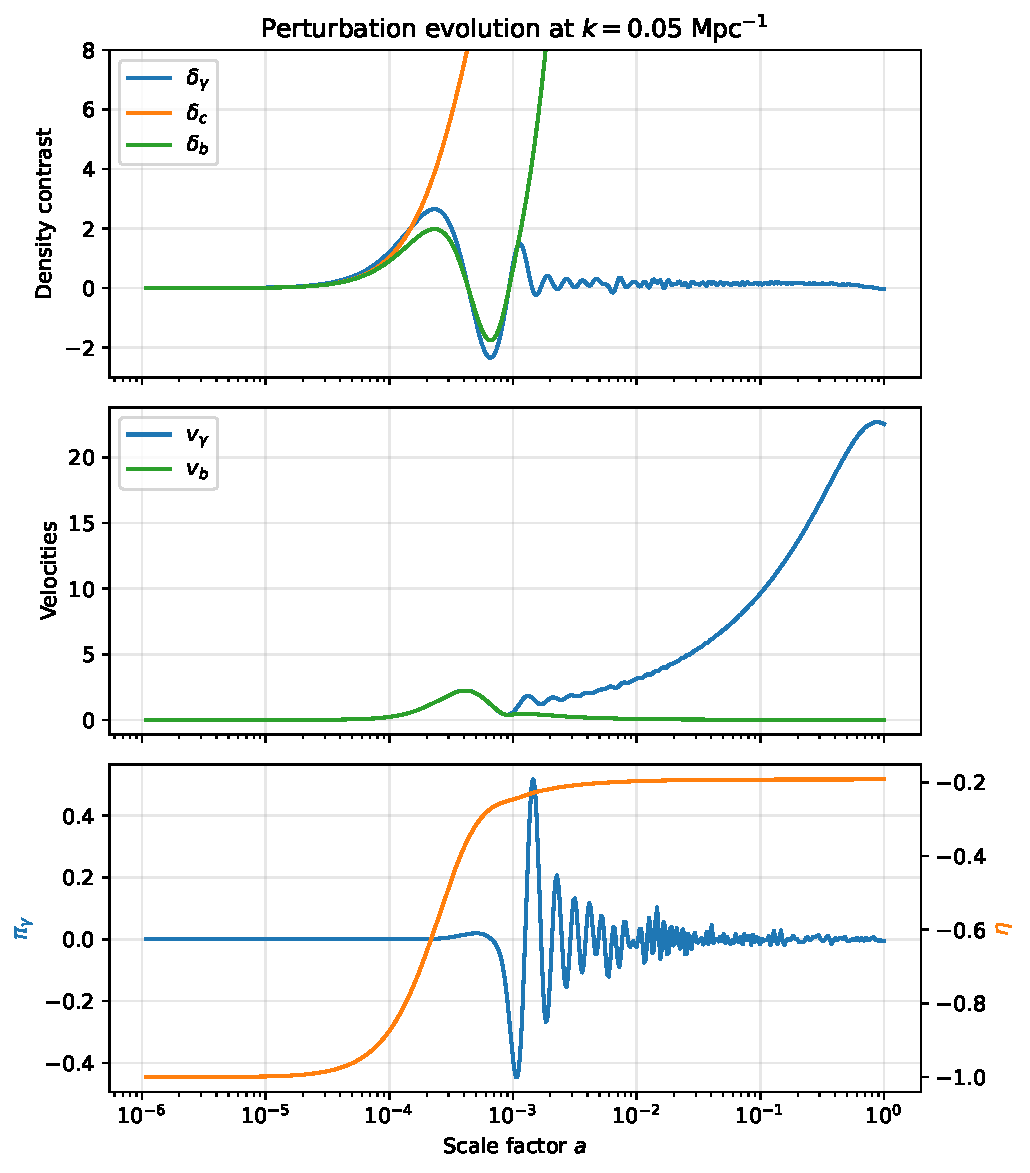
\includegraphics[width=0.95\linewidth]{figures/05_perturbations_k0p05.pdf}
\end{center}

\noindent Three panels, top to bottom:

\paragraph{Top -- densities.} On super-horizon scales (early $a$) all density contrasts evolve in lockstep at $\delta_i \propto a^2$: this is the adiabatic mode, with $\delta_c = \delta_b = (3/4)\delta_\gamma$. Once $k\tau \sim 1$ (horizon crossing, around $a \sim 10^{-4}$) the photon-baryon system starts to oscillate -- the acoustic oscillations we will project onto $C_\ell$ in chapter 5. $\delta_c$ keeps growing because CDM has no pressure. After recombination $\delta_b$ no longer feels the photon-pressure restoring force and falls into the dark-matter potential wells, eventually catching up to $\delta_c$.

\paragraph{Middle -- velocities.} The photon velocity $v_\gamma$ oscillates 90$^\circ$ out of phase with $\delta_\gamma$ (this is what a damped oscillator does). The baryon velocity tracks $v_\gamma$ very closely in the tight-coupling regime and decouples only at $a \approx 10^{-3}$, where you can see $v_b$ stop oscillating while $v_\gamma$ continues to grow (the photons free-stream after decoupling).

\paragraph{Bottom -- anisotropic stress and metric.} The photon anisotropic stress $\pi_\gamma$ is suppressed by tight coupling before recombination ($\pi_\gamma \ll \delta_\gamma$ in the high-opacity regime). It briefly oscillates during the recombination handoff and ringdowns afterward as photons free-stream. The synchronous-gauge metric variable $\eta$ approaches a constant on super-horizon scales -- this is what conservation of $\mathcal{R}$ outside the horizon looks like in this gauge -- then settles to a smaller value after horizon crossing.

\begin{physinsight}[Where the CMB is in this plot]
The CMB temperature anisotropy is, to leading order, the visibility-weighted value of $\Theta_0 + \Psi_W = \delta_\gamma/4 + \Psi_W$ at last scattering. The recombination time in the plot is around $a \sim 10^{-3}$ -- exactly where the photon density contrast shows its final acoustic oscillation before going silent. The value of $\delta_\gamma$ at $a \sim 10^{-3}$ for each $k$, weighted by $g(\tau)$ and projected onto the sphere with a $j_\ell(k\chi_*)$ kernel, becomes the temperature anisotropy on the corresponding angular scale. Everything in the rest of the tutorial is bookkeeping that turns these snapshot values into the angular power spectrum on our sky.
\end{physinsight}

\subsection{Looking ahead}

We have the perturbation evolution for a single $k$. To get to the CMB power spectrum we need to (i) extract source functions from the perturbations at each $k$ and $\tau$, (ii) project them through the spherical-Bessel kernel to get transfer functions $\Delta_\ell(k)$, and (iii) integrate $\Delta_\ell(k)^2$ against the primordial power spectrum to get $C_\ell$. The first step is the line-of-sight trick of chapter 4.
